%
%Не забыть:
%--------------------------------------
%Вставить колонтитулы, поменять название на титульнике



%--------------------------------------

\documentclass[a4paper, 12pt]{article} 

%--------------------------------------
%Russian-specific packages
%--------------------------------------
%\usepackage[warn]{mathtext}
\usepackage[T2A]{fontenc}
\usepackage[utf8]{inputenc}
\usepackage[english,russian]{babel}
\usepackage[intlimits]{amsmath}
\usepackage{esint}
%--------------------------------------
%Hyphenation rules
%--------------------------------------
\usepackage{hyphenat}
\hyphenation{ма-те-ма-ти-ка вос-ста-нав-ли-вать}
%--------------------------------------
%Packages
%--------------------------------------
\usepackage{amsmath}
\usepackage{amssymb}
\usepackage{amsfonts}
\usepackage{amsthm}
\usepackage{latexsym}
\usepackage{mathtools}
\usepackage{etoolbox}%Булевые операторы
\usepackage{extsizes}%Выставление произвольного шрифта в \documentclass
\usepackage{geometry}%Разметка листа
\usepackage{indentfirst}
\usepackage{wrapfig}%Создание обтекаемых текстом объектов
\usepackage{fancyhdr}%Создание колонтитулов
\usepackage{setspace}%Настройка интерлиньяжа
\usepackage{lastpage}%Вывод номера последней страницы в документе, \lastpage
\usepackage{soul}%Изменение параметров начертания
\usepackage{hyperref}%Две строчки с настройкой гиперссылок внутри получаеммого
\usepackage[usenames,dvipsnames,svgnames,table,rgb]{xcolor}% pdf-документа
\usepackage{multicol}%Позволяет писать текст в несколько колонок
\usepackage{cite}%Работа с библиографией
\usepackage{subfigure}% Человеческая вставка нескольких картинок
\usepackage{tikz}%Рисование рисунков
% Для картинок Моти
\usepackage{misccorr}
\usepackage{lscape}
\usepackage{cmap}


\usepackage{graphicx,xcolor}
\graphicspath{{Pictures/}}
\DeclareGraphicsExtensions{.pdf,.png,.jpg}

%----------------------------------------
%Список окружений
%----------------------------------------
\newenvironment {theor}[2]
{\smallskip \par \textbf{#1.} \textit{#2}  \par $\blacktriangleleft$}
{\flushright{$\blacktriangleright$} \medskip \par} %лемма/теорема с доказательством
\newenvironment {proofn}
{\par $\blacktriangleleft$}
{$\blacktriangleright$ \par} %доказательство
%----------------------------------------
%Список команд
%----------------------------------------
\newcommand{\grad}
{\mathop{\mathrm{grad}}\nolimits} %градиент

\newcommand{\diver}
{\mathop{\mathrm{div}}\nolimits} %дивергенция

\newcommand{\Def}[1]
{\underline{\textbf{#1}}} %определение

\newcommand{\RN}[1]
{\MakeUppercase{\romannumeral #1}} %римские цифры

\newcommand {\theornp}[2]
{\textbf{#1.} \textit{ #2} \par} %Написание леммы/теоремы без доказательства

\newcommand{\qrq}
{\ensuremath{\quad \Rightarrow \quad}} %Человеческий знак следствия

\newcommand{\qlrq}
{\ensuremath{\quad \Leftrightarrow \quad}} %Человеческий знак равносильности

\renewcommand{\phi}{\varphi} %Нормальный знак фи

\newcommand{\me}
{\ensuremath{\mathbb{E}}}

\newcommand{\md}
{\ensuremath{\mathbb{D}}}



%\renewcommand{\vec}{\overline}




%----------------------------------------
%Разметка листа
%----------------------------------------
\geometry{top = 3cm}
\geometry{bottom = 2cm}
\geometry{left = 1.5cm}
\geometry{right = 1.5cm}
%----------------------------------------
%Колонтитулы
%----------------------------------------
\pagestyle{fancy}%Создание колонтитулов
\fancyhead{}
%\fancyfoot{}
\fancyhead[R]{\textsc{Генератор Ван де Граафа}}%Вставить колонтитул сюда
%----------------------------------------
%Интерлиньяж (расстояния между строчками)
%----------------------------------------
%\onehalfspacing -- интерлиньяж 1.5
%\doublespacing -- интерлиньяж 2
%----------------------------------------
%Настройка гиперссылок
%----------------------------------------
\hypersetup{				% Гиперссылки
	unicode=true,           % русские буквы в раздела PDF
	pdftitle={Заголовок},   % Заголовок
	pdfauthor={Автор},      % Автор
	pdfsubject={Тема},      % Тема
	pdfcreator={Создатель}, % Создатель
	pdfproducer={Производитель}, % Производитель
	pdfkeywords={keyword1} {key2} {key3}, % Ключевые слова
	colorlinks=true,       	% false: ссылки в рамках; true: цветные ссылки
	linkcolor=blue,          % внутренние ссылки
	citecolor=blue,        % на библиографию
	filecolor=magenta,      % на файлы
	urlcolor=cyan           % на URL
}
%----------------------------------------
%Работа с библиографией (как бич)
%----------------------------------------
\renewcommand{\refname}{Список литературы}%Изменение названия списка литературы для article
%\renewcommand{\bibname}{Список литературы}%Изменение названия списка литературы для book и report
%----------------------------------------
\begin{document}
	\begin{titlepage}
		\begin{center}
			$$$$
			$$$$
			$$$$
			$$$$
			{\Large{НАЦИОНАЛЬНЫЙ ИССЛЕДОВАТЕЛЬСКИЙ УНИВЕРСИТЕТ}}\\
			\vspace{0.1cm}
			{\Large{ВЫСШАЯ ШКОЛА ЭКОНОМИКИ}}\\
			\vspace{0.25cm}
			{\large{Факультет физики}}\\
			\vspace{5.5cm}
			{\Huge\textbf{{Лабораторная работа}}}\\%Общее название
			\vspace{1cm}
			{\LARGE{<<Генератор Ван де Граафа>>}}\\%Точное название
			\vspace{2cm}
			{Работу выполнил студент 2 курса}\\
			{Захаров Сергей Дмитриевич}
			\vfill
			
\includegraphics[width = 0.2\textwidth]{HSElogo}\\
			\vfill
			Москва\\
			2019
		\end{center}
	\end{titlepage}

\tableofcontents

\newpage

\section{Цель работы}

Перед началом работы были поставлены следующие цели:

\begin{enumerate}
	\item Определить напряженность пробоя воздуха.
	
	\item Определить напряжение генератора Ван де Граафа, чтобы в дальнейшем получить напряженность пробоя воздуха альтернативным способом.
\end{enumerate}

\section{Описание метода выполнения работы}

%Тут будет схема

\subsection{Определение напряжения пробоя воздуха}

Сперва определимся с формулой, с помощью который мы будем это напряжение определять. Для этого обратимся к \cite{Jackson}, откуда получим формулу:

\begin{equation}
	\phi(x) = \frac{q}{|x - \left(r_l + d + r_b\right)|} - \frac{r_l}{r_l + d + r_b} \cdot \frac{q}{\left|x - \dfrac{r_l^2}{r_l + d + r_b}\right|}
\end{equation}

Здесь $r_l$ --- радиус меньшей сферы, $r_b$ --- радиус большей сферы, $d$ --- расстояние между ними.

\medspace

Чтобы получить разность потенциалов, зафиксируем точки, между которыми разность нужна. При этом, согласно устройству генератора, потенциал второй сферы равен нулю (она заземлена). В таком случае искомая разность потенциалов записывается в виде:

\begin{equation}
	\Delta \phi = \frac{q}{r_b} - \frac{r_l q}{\left|2 r_l d + r_l r_b + r_b d + d^2\right|}
	\label{phi_break_bad}
\end{equation}

\medspace

Теперь учтем, что заряд может быть выражен как $q = I T$, где $I$ --- ток генератора, $T$ --- период искрового разряда и получим из (\ref{phi_break_bad}) финальную формулу:

\begin{equation}
	\Delta \phi = \frac{IT}{r_b} - \frac{r_l IT}{\left|2 r_l d + r_l r_b + r_b d + d^2\right|}
	\label{phi_break_better}
\end{equation} 

Здесь $I$ --- ток генератора, $T$ --- период искрового разряда, $r_b$ --- радиус большой сферы, $r_l$ --- радиус маленькой сферы, $d$ --- расстояние между сферами.

\medspace

Измерить радиусы сфер и расстояние между сферами не представляет большого труда.

Измерение тока было решено провести косвенно, замерив напряжение на известном сопротивлении. В таком случае ток можно выразить через сопротивление по закону Ома:

\begin{equation}
	I = \frac{U}{R}
	\label{Om}
\end{equation}

Здесь $U$ --- напряжение на сопротивлении, $R$ --- его величина.

\medspace

Таким образом формула (\ref{phi_break_better}) преображается в вид:

\begin{equation}
	\Delta \phi = \frac{UT}{Rr_b} - \frac{r_l UT}{R \cdot \left|2 r_l d + r_l r_b + r_b d + d^2\right|}
	\label{phi_break_best}
\end{equation}

\medspace

Чтобы определить период искрового разряда, к генератору был поднесен щуп осциллографа, который улавливал наводки. Период этих наводок совпадал с периодом искрового разряда.

\subsection{Определение напряжение генератора Ван де Граафа}

Для того, чтобы измерить напряжение генератора, можно воспользоваться следующим приближением: пренебрежем различиями сфер в размерах. В таком случае наш генератор фактически является шаровым разрядником. Для такого объекта существует таблица, связывающая диаметр шаров и расстояние между ними с напряжением пробоя воздуха между шарами, которое в то же время равняется и напряжению шара \cite{GOST}.

%Напрямую измерить напряжение на генераторе возможным, к сожалению, не представляется, потому что оно может сжечь измерительные приборы. %Ссу в уши, плохо звучит
%По этой причине было решено воспользоваться методом измерения с помощью шаровых разрядников. Мы пренебрегли тем, что шары имеют различные размеры, и свели наш генератор как раз к шаровому разряднику. Для него же существует таблица, связывающая диаметр шаров и расстояние между ними с напряжением пробоя воздуха между шарами, которое в то же время равняется и напряжению шара \cite{GOST}.

Согласно ГОСТу, чтобы получить действительное напряжение пробоя, необходимо данные из таблицы, приведенной в нем, умножить на коэффициент, равный относительной влажности воздуха $\rho$ (при условии, что она лежит в промежутке $\rho\in [0.95; 1.05]$), которая в свою очередь рассчитывается следующим образом:

\begin{equation}
	\rho = 0.386 \cdot \frac{P}{273^\circ \text{C}+ t} %хз про размерность
	\label{Coefficient}
\end{equation}

Здесь $P$ --- атмосферное давление (в миллиметрах ртутного столба), $t$ --- температура окружающей среды.

\section{Выполнение работы}

Сперва были замерены следующие величины, необходимые в работе:

\medspace

\begin{tabular}{|c|c|c|c|}
	\hline 
	Сопротивление $R_1$, ГОм & Сопротивление $R_2$, кОм & $r_l$, см & $r_b$, см \\ 
	\hline 
	$3.3 \pm 0.165 $& $110 \pm 1$   & $5.5 \pm 0.05$ & $11.28 \pm 0.1$ \\ 
	\hline
\end{tabular} 

\medspace

Затем было получено, что зависимость напряжения на резисторе $R_2$ от напряжения на источнике в целом является линейной начиная с напряжения 3~В на последнем. Это отчетливо видно на рисунке (\ref{Voltage_graphic}). По этой причине, зная напряжение на источнике, представляется возможным определить напряжение на резисторе $R_2$ следующим образом:

\begin{equation}
	U_{R_2} =  U \cdot 0.116 - 0.246 \text{  В}
	\label{UR}
\end{equation}

Напряжение источника $U$ подставляется в вольтах.

\begin{figure}[ht!]
	\center
	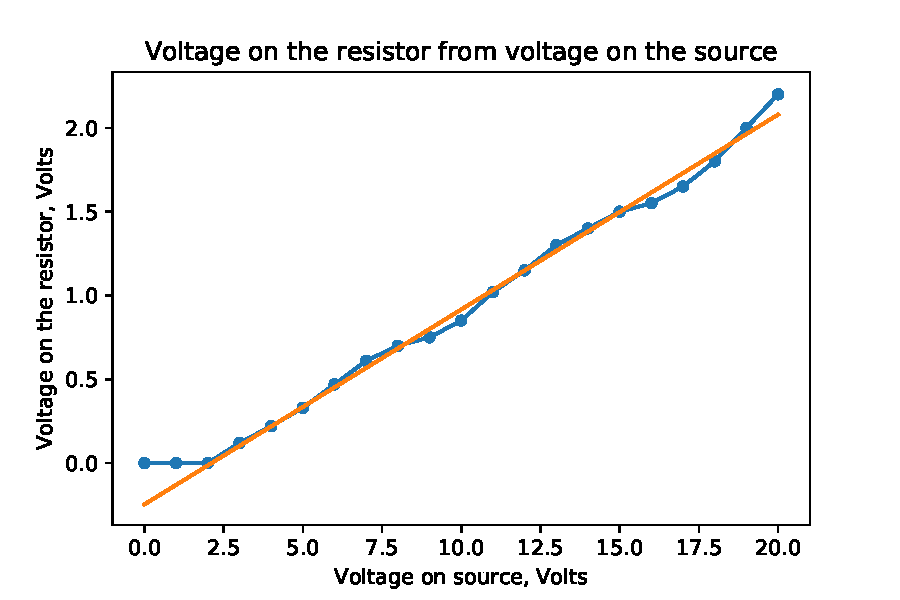
\includegraphics[width=0.7\textwidth]{Voltage}
	\caption{Зависимость напряжения на резисторе 110~кОм от напряжения на источнике}
	\label{Voltage_graphic}
\end{figure}

После этого были проведены измерения зависимости периода разряда от расстояния между шарами при двух напряжениях на источнике: 8 В и 11 В. Результаты измерений представлены на рисунке \ref{fig:TV}. В целом видно, что их можно аппроксимировать линейной функцией.

\begin{figure}[ht!]
	\centering
	\subfigure[]{
	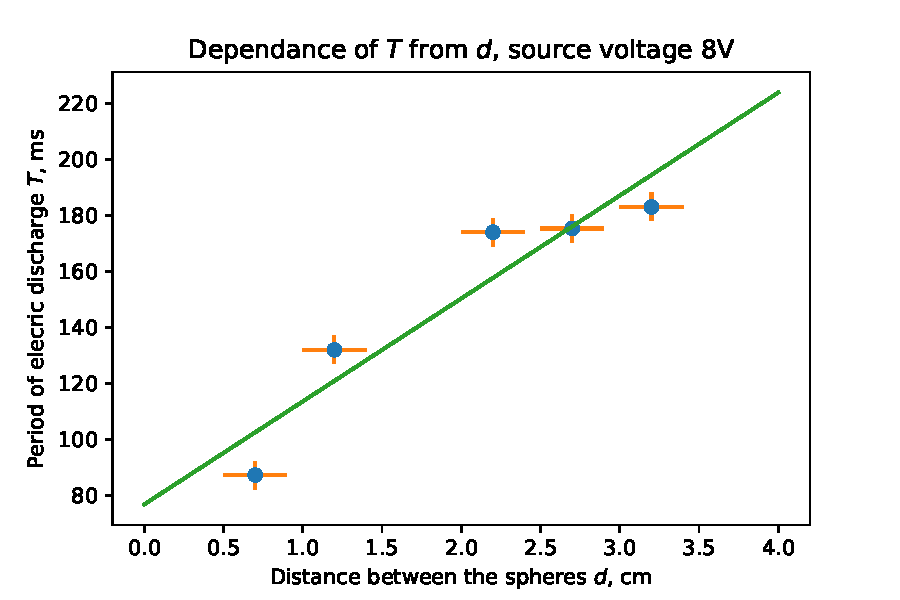
\includegraphics[width=0.48\linewidth]{8V}
	\label{fig:T8V}}
	\subfigure[]{
	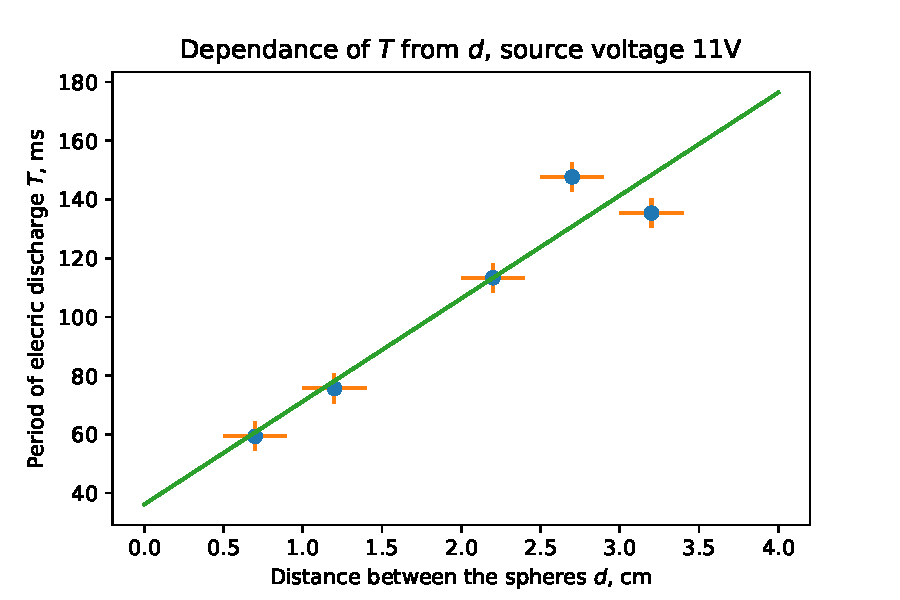
\includegraphics[width=0.48\linewidth]{11V}
	\label{fig:T11V}}
	\caption{Зависимость периода разряда от расстояния между сферами при напряжении на источнике 8~В \subref{fig:T8V} и 11~В \subref{fig:T11V}}
	\label{fig:TV}
\end{figure}

После того, как мы получили периоды, мы, наконец, можем рассчитать разность потенциалов между сферами по формуле (\ref{phi_break_best}), а с ней и напряженность в предположении, что поле между сферами однородное, а значит $E = \Delta \phi / d$. Полученные данные отображены на рисунке \ref{fig:E}.

\begin{figure}[h]
	\centering
	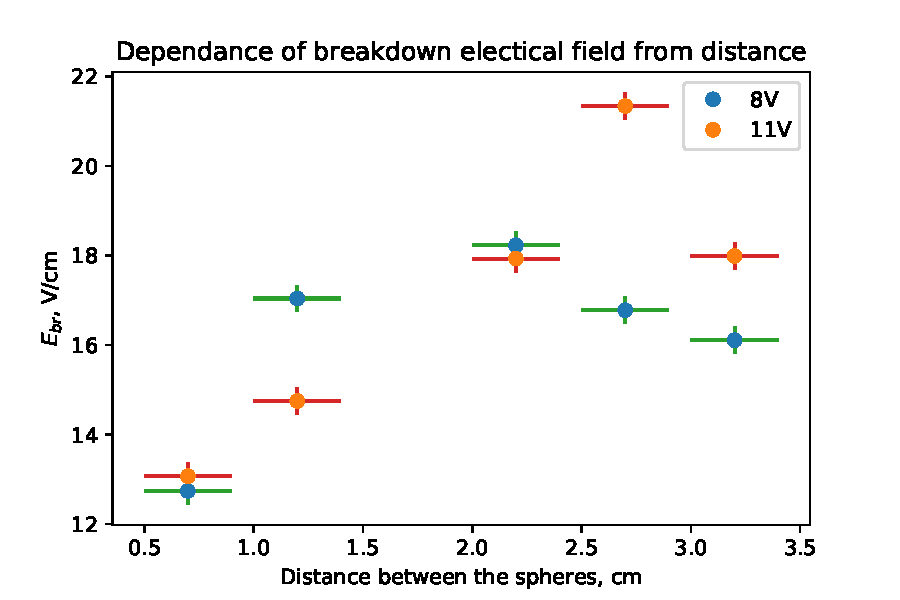
\includegraphics[width=0.8\linewidth]{E}
	\caption{Зависимость напряженности пробоя воздуха от расстояния между сферами при напряжении 8~В и 11~В}
	\label{fig:E}
\end{figure}

Проведя усреднение по всем имеющимся данным, получаем, что напряженность пробоя воздуха приблизительно равна \boxed{E_{br} = 16.6 \pm 0.3 \text{~кВ/см}}.

\bigskip

Теперь перейдем ко второму пункту задания. Воспользовавшись формулой (\ref{Coefficient}) при условии, что температура в помещении была около 27$^\circ$C, а атмосферное давление 746 мм. рт. ст., получаем, что коэффициент перевода оказывается равен $\rho = 0.86$. На основании данных из таблицы в \cite{GOST} получаем, что напряженность пробоя должна быть около 24~кВ/см.

\section{Анализ результатов}

Как видно, полученное значение напряженности отличается от того, которое должно быть в реальности. Это можно объяснить следующими факторами, которые не были учтены в ходе выполнения работы:

\begin{enumerate}
	\item При возникновении разряда сферы начинали колебаться, что фактически вносило дополнительные поправки в измерение расстояния между сферами
	
	\item Провода в работе были далеко не высоковольтными, что означает, что потенциально могли возникать неучтенные утечки.
	
	\item При выполнении работы возникали постоянные паразитные наводки, связанные с работой нескольких генераторов одновременно.
	
\end{enumerate}




\newpage


\begin{thebibliography}{9}
	\addcontentsline{toc}{section}{\refname}
	\bibitem{GOST} ГОСТ 17512-82 (СТ СЭВ 2732-80). Электрооборудование и электроустановки на напряжение 3 кВ и выше. Методы измерения при испытаниях высоким напряжением. -- 1982
	
	\bibitem{Jackson} Jackson J. D. Classical Electrodynamics. New York: John Wiley and Sons, 1965. 702 p.
\end{thebibliography}










\end{document}





















